\section{Bloc mémoire}

\indent Cette première partie traite de la génération du bloc mémoire fonctionnel. L'objectif est d'obtenir un bloc contenant un nombre générique de mémoires ainsi qu'un décodeur pour en gérer l'accès, via des signaux \textit{Chip Select}.

\subsection{Récupération d'une IP de RAM}

\indent Il nous a été fourni un modèle simple de mémoire RAM. La première tache vise à coprendre son fonctionnement puis de trouver une solution afin de rendre son implémentation générique tant sur la taille des données que sur l'adresse.

\begin{figure}[h]
	\centering
	\includegraphics[width=0.97\linewidth]{bloc\_ram.png}
	\caption{Bloc RAM niveau RTL}
	\label{fig:synth_bloc_ram}
\end{figure}

\indent Après modification du modèle, nous avons pu générer deux bancs de test avec Cocotb qui consistent à tester l'écriture via le signal \textit{Write Enable (we)} et l'activation selon le signal \textit{Chip Select (cs)}.

\begin{figure}[h]
	\centering
	\includegraphics[width=0.97\linewidth]{ramchip\_wave.png}
	\caption{Simulation du bloc mémoire}
	\label{fig:wave_bloc_ram}
\end{figure}

\newpage

\subsection{Décodeur d'adresse}

\indent En vue de pouvoir intégrer plusieurs instances de la RAM, il est nécessaire de décrire un décodeur d'adresses qui analysera les n-bits de poids fort (n pour la généricité) pour accéder aux différentes RAM en lecture ou en écriture.

\begin{figure}[h]
	\centering
	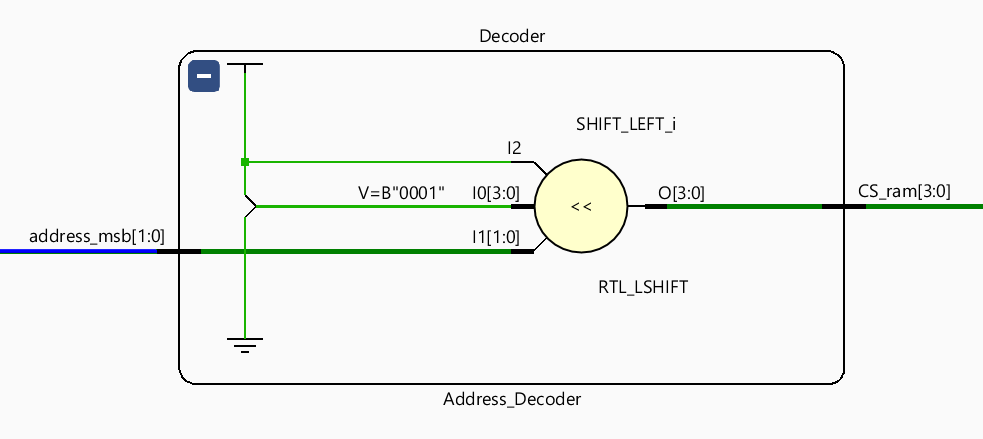
\includegraphics[width=0.97\linewidth]{decodeur.png}
	\caption{Décodeur au niveau RTL}
	\label{fig:synth_bloc_decodeur}
\end{figure}

\indent Le décodeur fonctionne de façon purement combinatoire et le banc de test est élémentaire: il suffit de tester les 2**n entrées possibles, n étant le nombre de vits de poids fort pris en considération. Via l'utilisation de Cocotb, il est aisé de vérifier les sorties pour des n différents (ci-dessous, les tests pour n = 2 et n = 3).

\begin{figure}[h]
	\centering
	\begin{subfigure}{0.3\textwidth}
		\includegraphics[width=\textwidth]{decoder\_entry\_2\_out.png} 
	\end{subfigure}
	\hfill
	\begin{subfigure}{0.3\textwidth}
		\includegraphics[width=\textwidth]{decoder\_entry\_3\_out.png}
	\end{subfigure}
	\caption{Tableau d'entrées/sorties du décodeur pour 2 et 3 bits de poids fort en entrée}
	\label{fig:stdout_decoder_2_3}
\end{figure}


\begin{figure}[h]
	\centering
	\includegraphics[width=0.97\linewidth]{decoder\_entry\_2\_wave.png}
	\caption{Simulation du décodeur pour 2 bits de poids fort en entrée}
	\label{fig:wave_bloc_decoder}
\end{figure}

\newpage

\subsection{Bloc Quad-ram}

\indent Le bloc Quadram est le top module du bloc mémoire. Il ne contient en réalité que des générations d'instances de RAM et du décodeur, toujours d'une façon générique suivant la taille du bus d'adresse et du bus de données. Il n'est pas possible de déterminer manuellement le nombre de bloc RAM instancié, celui-ci est en effet calculé suivant le nombre de bits de poids forts pris en compte.

\begin{figure}[h]
	\centering
	\includegraphics[width=0.97\linewidth]{bloc\_quadram.png}
	\caption{Bloc mémoire complet niveau RTL}
	\label{fig:synth_bloc_quadram}
\end{figure}

\indent Nous avons ensuite pu générer un banc de tests avec Cocotb qui consistent à faire un cycle de 10 écritures à des adresses aléatoires en mémoire puis de faire 10 cycles de lecture à ces mêmes adresses pour vérifier le contenu des blocs RAM et le fonctionnement des signaux \textit{Chip Select}.

\begin{figure}[h]
	\centering
	\includegraphics[width=0.97\linewidth]{quadram\_wave.png}
	\caption{Simulation du bloc mémoire complet}
	\label{fig:wave_bloc_quadram}
\end{figure}

\indent Le nom donné par défaut est "Quadram" mais en réalité le modèle pourrait en contenir 1, 2, 8, 16 ...

